\documentclass[conference]{IEEEtran}
\IEEEoverridecommandlockouts
\usepackage{cite}
\usepackage{amsmath,amssymb,amsfonts}
\usepackage{graphicx}
\usepackage{textcomp}
\usepackage{xcolor}
\usepackage{booktabs}
\usepackage{multirow}
\usepackage{url}
\usepackage{array}

% Decision states are labels, not products of variables: keep them upright.
\newcommand{\dstate}[1]{\ensuremath{\mathrm{#1}}}
% Indicator function. \mathbb{1} is not available in msbm (it renders as a
% stray relation symbol), so the indicator is set with a bold upright 1.
\newcommand{\ind}{\mathbf{1}}

\begin{document}

\title{Uncertainty-Aware Multimodal Evidence Fusion for
Vessel-Associated Subsea Cable Disturbance Assessment}

\author{
\IEEEauthorblockN{Dr.A.Syed Musthafa\IEEEauthorrefmark{1}}
\IEEEauthorblockA{Department of Information Technology\\
M Kumarasamy College of Engineering\\
Karur, India\\
sathiyanathans@mkce.ac.in}
\and
\IEEEauthorblockN{Muthukrishnan C}
\IEEEauthorblockA{Department of Information Technology\\
M Kumarasamy College of Engineering\\
Karur, India\\
muthukrishnanchellamuthu8893@gmail.com}
\and
\IEEEauthorblockN{Muthuvel Mukesh K}
\IEEEauthorblockA{Department of Information Technology\\
M Kumarasamy College of Engineering\\
Karur, India\\
muthuvelmukesh0609@gmail.com}
\and
\IEEEauthorblockN{Shanmugavel M}
\IEEEauthorblockA{Department of Information Technology\\
M Kumarasamy College of Engineering\\
Karur, India\\
mshanmugavel065@gmail.com}
\thanks{\IEEEauthorrefmark{1}Corresponding author.}
}

\maketitle

\begin{abstract}
Subsea cables are critical international infrastructure, yet detecting a
seafloor vibration anomaly establishes neither that a vessel produced it nor
that the cable was damaged. This paper presents an
uncertainty-aware multimodal evidence fusion framework that separates physical
detection, spatio-temporal association, vessel kinematics, sensor health, and
counter-evidence into distinct streams, combined through a fail-closed decision
hierarchy with operational states \dstate{T0}--\dstate{T3}
and a degraded-evidence state \dstate{TX}. We evaluate it on three real
submarine distributed acoustic sensing (DAS) records: an Automatic
Identification System (AIS)-linked container-ship transit (Marlinks), a deep-sea
background recording (EMSO Western Ionian), and a 27.625-day Arctic recording
(Dryad Oliktok). On Marlinks, DAS separates 1~km corridor incursions with an
area under the receiver operating characteristic curve (AUC) of $0.959$ (95\%
CI $[0.887, 1.000]$), and DAS power tracks AIS range at Spearman
$\rho=-0.948$. The framework produced zero false escalations on 85/85 EMSO
background windows and all 215 Oliktok windows, whose noise floor was stable
(drift $+0.0188/\mathrm{hr}$) and tracked independent wave height. The adversarial evasion rate against four AIS
manipulation families at five severities is $0.0$. As a negative result, the
full framework attains lower escalation F1 ($0.462$ real, $0.235$ simulated)
than simple weighted fusion ($0.824$, $0.333$): the system is tuned to fail
closed rather than to maximize recall. End-to-end latency averages 8.289~ms.
Detection, association, and attribution are evaluated as separate claims
throughout, each checked against real submarine DAS data.
\end{abstract}

\begin{IEEEkeywords}
subsea cable protection, distributed acoustic sensing, Automatic
Identification System, multimodal sensor fusion, uncertainty estimation, critical infrastructure,
adversarial robustness, environmental robustness, reproducibility
\end{IEEEkeywords}

\section{Introduction}

Subsea fiber-optic telecommunication cables and submarine high-voltage power
cables underpin modern global connectivity and energy security. Unscheduled
outages cause major societal and economic disruption. Autonomous monitoring is
critical for rapid anomaly detection; however, determining whether an observed
seafloor disturbance is caused by external human activity remains challenging.

Commercial shipping and fishing activities represent prominent maritime
hazards. Anchoring, bottom trawling, and vessel maneuvering can generate intense
vibrations near submerged cables. Nevertheless, vibration signals captured along
a seafloor fiber do not speak for themselves. An acoustic or strain anomaly may
arise from vessel interaction, ambient hydrodynamic forcing (surface gravity
waves, microseisms), non-vessel seabed mechanical disturbances, or optical
interrogator drift. Consequently, this investigation formalizes and enforces
the operational principle:
\begin{equation}
\text{Detection} \neq \text{Association} \neq \text{Attribution}.
\label{eq:principle}
\end{equation}
Physical \emph{detection} identifies whether a significant energetic deviation
occurred on the fiber. Spatio-temporal \emph{association} tests whether that
deviation is spatially proximate and temporally synchronized with an external
event (such as a transiting vessel). Causal \emph{attribution} determines
whether the totality of evidence justifies assigning responsibility to a
specific external agent or mechanism.

As demonstrated in Section~\ref{sec:real-results}, physical detection alone is
incapable of supporting safe protection decisions: on real submarine DAS data, a
transiting cargo ship induces measurable optical strain out to 1.5~km, meaning a
physical-only detector triggers in every window, achieving a recall of 1.000 but
a precision of only 0.526 against a 1~km security corridor.

A further complication arises under adversarial conditions. Automated
Identification System (AIS) transponders are unauthenticated and vulnerable to
vessel-side manipulation, including GPS spoofing, intentional transponder
deactivation, timestamp alteration, and false spatial reporting. A fusion
system that unreservedly trusts vessel broadcasts can be deceived into
ignoring real physical incursions or falsely escalating benign transits.
The monitoring framework must therefore operate under bounded adversarial
uncertainty as well as natural environmental variability.

\subsection{Scope and Validation Status}
\label{sec:scope-detail}

To maintain rigorous scientific integrity, this paper reports experimental
outcomes strictly for executed modules, using traceable hashes and verified
manifests. Four validation components were defined across this research:
(i) controlled synthetic simulation over 22 benchmark scenarios (2,200 trials);
(ii) real-world validation against real submarine DAS and AIS records;
(iii) long-duration real-DAS environmental robustness validation against
independent Arctic oceanographic moorings; and (iv) physical hardware-in-the-loop
validation with ESP32--MPU6050 sensor nodes.

Components (i), (ii), and (iii) were executed and are reported with exact
numerical metrics. Component (iv) was not physically constructed;
Section~\ref{sec:hardware} details its proposed architectural scope, what
empirical quantities it would measure, and what scientific claims it would and
would not license. Table~\ref{tab:status} summarizes the validation status.

\begin{table}[!t]
\caption{Validation Status of the Evaluated and Proposed Framework Components}
\label{tab:status}
\centering
\footnotesize
\setlength{\tabcolsep}{3pt}
\begin{tabular}{@{}>{\raggedright\arraybackslash}p{0.34\columnwidth}>{\raggedright\arraybackslash}p{0.30\columnwidth}>{\raggedright\arraybackslash}p{0.26\columnwidth}@{}}
\toprule
Component & Evidence / Scope & Status \\
\midrule
Controlled simulation (S01--S22) & 2{,}200 seeded trials & \textbf{EXECUTED} \\
Real DAS + AIS transit (Dataset A) & 60 windows, 250 ch & \textbf{EXECUTED} \\
Real DAS background (Dataset B) & 105 windows, 2{,}963 ch & \textbf{EXECUTED} \\
Real DAS environmental (Dataset C) & 215 windows, 183 ch, 27.6~d & \textbf{EXECUTED} \\
Adversarial sweep on vessel AIS & 4 families $\times$ 5 sev. & \textbf{EXECUTED} \\
ESP32--MPU6050 testbed & Bench hardware build & FUTURE (Sec.~\ref{sec:hardware}) \\
Multi-vessel / damaged cable DAS & External incident logs & NOT EXECUTED \\
\bottomrule
\end{tabular}
\end{table}

The primary scientific contributions are:
\begin{enumerate}
\item An uncertainty-aware multimodal evidence fusion architecture that
separates physical detection from spatio-temporal association, vessel behavior,
sensor health, and uncertainty estimation, employing a fail-closed graded
decision model (\dstate{T0}--\dstate{T3}, \dstate{TX}).
\item A spatially coherent detection statistic whose operational threshold is
calibrated on an independent deep-sea background record rather than evaluation
splits, delivering a measured background false-alarm rate.
\item An adversarial cross-consistency check that contrasts DAS-derived range
inversion against vessel-broadcast AIS ranges, preventing vessel-side
falsification from silently forcing benign classifications.
\item Comprehensive empirical validation across three distinct real submarine
DAS deployments (Belgian North Sea, Western Ionian Sea, and Arctic Beaufort
Sea) comprising over 27.6 days of continuous acoustic recording, verifying
spatial decay, deep-sea stationarity, and oceanographic wave coupling.
\item Complete backward compatibility across 22 benchmark scenarios (22/22
identical decisions) under the updated reliability-first decision hierarchy,
resolving quiet-baseline misclassifications.
\item A transparent accounting of negative and bounded findings: at reference
thresholds, the full framework is outperformed on escalation F1 by simple
weighted fusion on both simulated and real data (evaluated independently).
The full framework is deliberately conservative: it is tuned to fail closed.
\end{enumerate}

\section{Related Work}

\subsection{Subsea Cable Monitoring and Sensing}
Structural health monitoring of underwater power and communication cables has
historically relied on Remotely Operated Vehicles (ROVs), sensing coil arrays,
and optical time-domain reflectometry \cite{b1,b2,b3,b4}. While vital for
post-fault localization and periodic inspection, these modalities do not provide
continuous real-time surveillance of external surface activities.

\subsection{Submarine Distributed Acoustic Sensing (DAS)}
Distributed acoustic sensing (DAS) interrogates standard optical fiber cables using
coherent optical time-domain reflectometry ($\Phi$-OTDR), transforming tens of
kilometers of subsea glass into dense arrays of dynamic strain sensors. Recent
studies have demonstrated submarine DAS for seismic recording, ocean wave
dynamics, and opportunistic surface vessel tracking \cite{b11,b12,b13,b14,b15}.
Most existing studies focus on raw acoustic processing, beamforming, or inverse
range modeling as standalone objectives. In contrast, this paper treats DAS as
one constituent of a heterogeneous, uncertainty-aware evidence fusion framework.

\subsection{AIS Integrity and Maritime Anomaly Detection}
The Automatic Identification System (AIS) provides kinematic vessel state
broadcasts used globally for maritime collision avoidance and traffic monitoring
\cite{b5,b6,b7}. However, AIS relies on unencrypted radio broadcasts lacking
cryptographic authentication. Vessels engaged in illicit activities frequently
disable transponders, spoof Maritime Mobile Service Identity (MMSI) numbers, or introduce deliberate GPS
offsets. AIS cannot serve as an unquestioned ground-truth oracle; its reports
must be validated against physically independent subsea sensing streams.

\subsection{Evidence Fusion under Conflict and Uncertainty}
Classical evidence fusion frameworks, such as Dempster--Shafer theory and
Dezert--Smarandache theory, provide mathematical foundations for combining
beliefs from disparate sensors. Under severe conflict, however, naive
combination rules produce counter-intuitive and volatile results \cite{b8,b9,b10}.
Recent methods introduce reliability weighting, distance-based conflict
discounting, and explicit uncertainty modeling. Our architecture integrates
sensor availability, physical health, and adversarial consistency into a
fail-closed decision engine.

\section{Problem Formulation}

Let $X = \{X_1, \ldots, X_N\}$ represent multimodal observations collected
across temporal sliding windows, where each observation possesses a sensor tag
and timestamp. We evaluate four competing hypotheses:
\begin{align}
H_1&: \text{vessel-associated subsea disturbance}, \\
H_2&: \text{environmental / hydrodynamic disturbance}, \\
H_3&: \text{non-vessel mechanical seabed disturbance}, \\
H_4&: \text{sensor degradation or interrogator fault}.
\end{align}
The decision rule maps the evidence space into a discrete operational state:
\begin{equation}
D = f(E^{+}, E^{-}, H, U, A),
\end{equation}
where $E^{+}$ represents supporting evidence, $E^{-}$ represents counter-evidence,
$H$ is the hypothesis space, $U \in [0, 1]$ is quantified uncertainty, and
$A \in [0, 1]$ represents sensor data availability.

\subsection{Adversarial Threat Model}
Let $X_{H_1}$ denote genuine observations generated during a true
vessel-associated interaction. An adversary seeking to conceal their presence
manipulates the vessel-side communication stream within an adversarial budget
$\Omega$, producing perturbed observations $\tilde{X}$. The threat model
specifically addresses vessel-side AIS and transponder manipulation:
(i) range inflation (reporting coordinates farther from the cable);
(ii) transponder suppression (omitting transmission bursts); (iii) timestamp
manipulation (injecting artificial transmission latencies); and (iv) combined
multi-vector evasion.

The threat model explicitly \emph{excludes} physical tampering with the subsea
fiber, optical interrogator firmware modification, and compromise of terrestrial
telecommunication networks. The foundational safety property is:
\begin{equation}
\forall \tilde{X} \in \Omega(X_{H_1}): D(\tilde{X}) \neq \dstate{T0}.
\label{eq:safety}
\end{equation}
The framework does not guarantee that every adversarial scenario escalates to
\dstate{T3}; rather, when evidence is corrupted or conflicting, it must degrade
to \dstate{TX} (insufficient / conflicting evidence) and strictly avoid collapsing
to \dstate{T0} (normal unperturbed baseline).

\section{Proposed Framework}

The architecture (Fig.~\ref{fig:architecture}) processes raw DAS phase strain
rates and AIS kinematic broadcasts through independent feature extraction
pipelines before performing spatio-temporal association, sensor health
validation, adversarial consistency verification, uncertainty estimation, and
graded decision output:
\begin{equation}
C_P \rightarrow (C_S, C_T, C_B) \rightarrow C_A \rightarrow R \rightarrow U \rightarrow D,
\end{equation}
where $C_P$ is physical disturbance confidence, $C_S, C_T, C_B$ denote spatial,
temporal, and behavioral association confidences, $C_A$ is composite association
confidence, $R$ is fused evidence reliability, $U$ is composite uncertainty, and
$D$ is the final decision state.

\begin{figure}[!t]
\centering
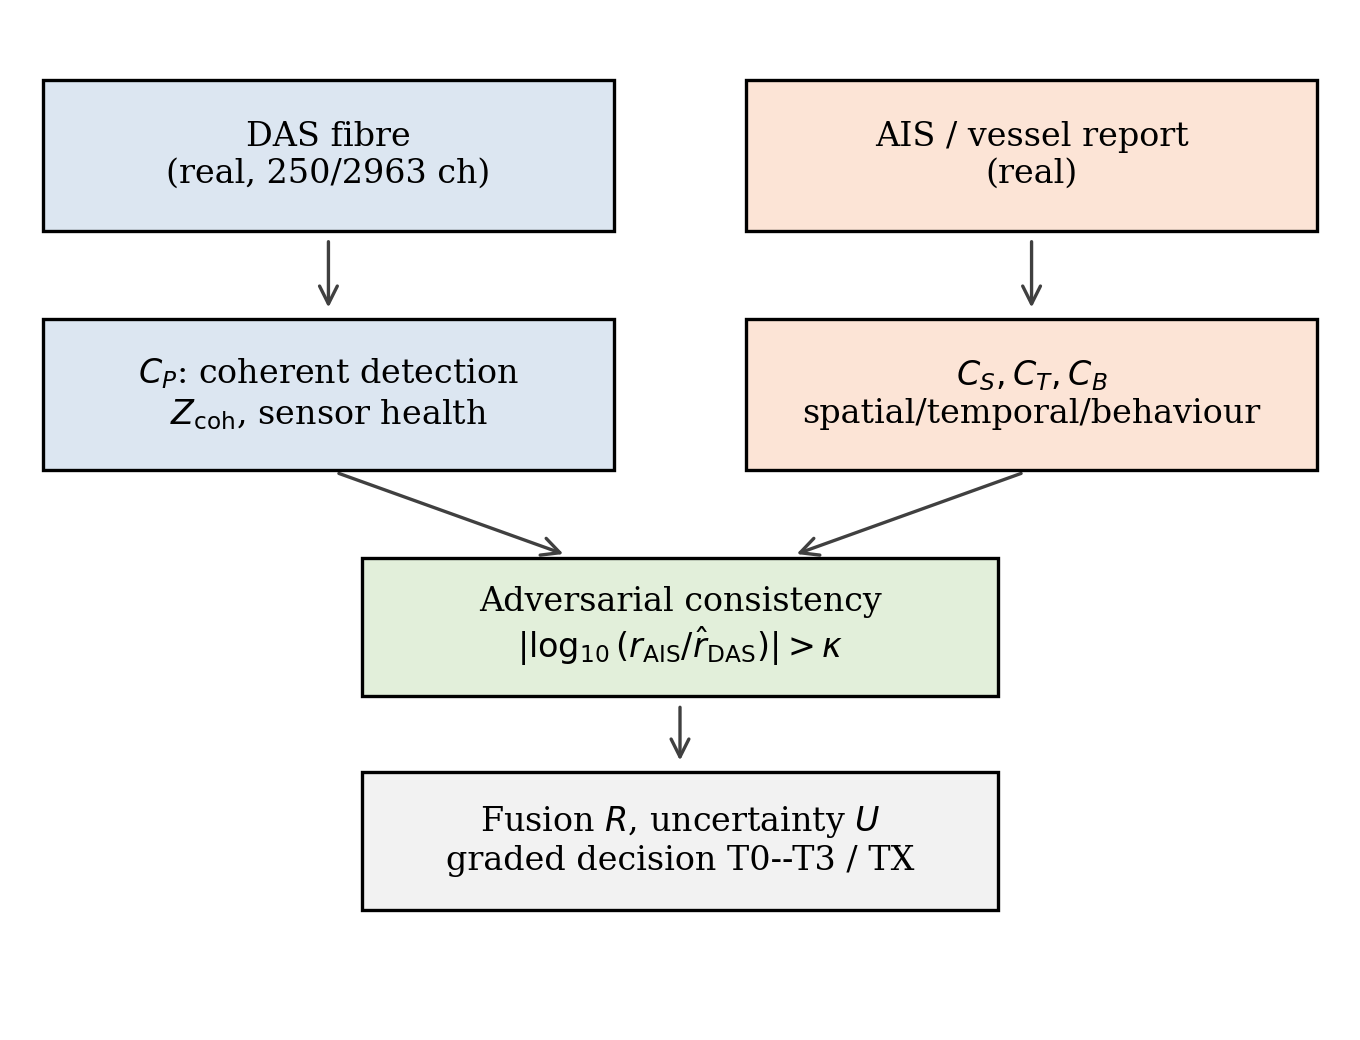
\includegraphics[width=0.46\textwidth]{figs/fig_architecture.png}
\caption{Processing architecture. The optical DAS strain pipeline and AIS
vessel telemetry remain strictly separated until the adversarial consistency
check, preventing vessel-side falsification from corrupting physical detection.}
\label{fig:architecture}
\end{figure}

\subsection{Physical Disturbance Detection}
For spatial channel $i$, the primary window feature is the root-mean-square
(RMS) strain amplitude $A_i = \sqrt{\frac{1}{n}\sum_s x_{i,s}^2}$. Per-channel
mean $\mu_i$ and standard deviation $\sigma_i$ are estimated over quiescent
baseline periods, yielding the standardized anomaly score $z_i = |A_i - \mu_i| / \sigma_i$.

Because isolated optical noise excursions or fading spikes can produce extreme
$z$-scores on individual channels, a channel-level threshold cannot control the
cable-level false-alarm rate across thousands of channels. True seabed
disturbances propagate elastically across multiple adjacent channels. The
cable-level detection statistic is thus formulated as the maximum $L$-channel
moving spatial average:
\begin{equation}
Z_{\mathrm{coh}} = \max_j \frac{1}{L}\sum_{i=j}^{j+L-1} z_i,
\qquad
C_P = \mathrm{sig}\!\left(\frac{Z_{\mathrm{coh}} - \tau_P}{k_P}\right),
\label{eq:zcoh}
\end{equation}
where $\mathrm{sig}(v) = 1/(1+e^{-v})$. The window length $L$ and detection
threshold $\tau_P$ are fixed strictly using independent baseline data disjoint
from evaluation splits.

\subsection{Spatial and Temporal Association}
Spatial proximity confidence is $C_S = \max(0, 1 - d/d_{\max})$, where $d$ is
the estimated distance from the vessel to the cable array and $d_{\max}$ is the
surveillance corridor radius. Temporal synchronization confidence is
$C_T = \max(0, 1 - |\Delta t| / t_{\max})$, where $\Delta t$ is the latency
between acoustic energy onset and the vessel's closest point of approach
(CPA) time. Rather than adopting an
arbitrary temporal tolerance, $t_{\max}$ is dynamically parameterized by vessel
kinematics as $t_{\max} = d_{\max} / v$, where $v$ is vessel speed over ground.

\subsection{Vessel Behavior and Sensor Health Weighting}
Behavioral risk confidence is computed over normalized kinematic features
$\phi_k(v)$ (speed anomalies, rate of turn, course changes):
$C_B = \mathrm{sig}\!\left(\sum_k b_k \phi_k(v)\right)$. Composite association
confidence combines these components: $C_A = \alpha C_S + \beta C_T + \gamma C_B$,
with $\alpha + \beta + \gamma = 1$.

Sensor health $H_i = 1 - \max_k(\rho_k \psi_k(i))$ evaluates hardware integrity
across degradation indicators $\psi_k$ (flatlined channels, optical saturation,
non-finite samples). Using availability $V_i \in [0, 1]$ and assigned weights
$w_i$, the fused evidence score is:
\begin{equation}
R = \frac{\sum_i w_i H_i V_i C_i}{\sum_i w_i H_i V_i + \epsilon}.
\end{equation}
Degraded or missing sensors therefore cannot artificially inflate confidence.

\subsection{Adversarial Range Consistency Check}
A vessel manipulating its AIS broadcast to conceal proximity displaces its
reported range $r_{\mathrm{AIS}}$ while leaving the seafloor acoustic strain
unaffected. The DAS array provides an independent physical range estimate
$\hat{r}_{\mathrm{DAS}}$. The consistency check triggers when the reported range
is significantly larger than the acoustic estimate during an active disturbance:
\begin{equation}
\log_{10}\!\left(\frac{r_{\mathrm{AIS}}}{\hat{r}_{\mathrm{DAS}}}\right) > \kappa
\ \wedge\ C_P \geq \theta_P \;\Rightarrow\; \dstate{TX}.
\label{eq:consistency}
\end{equation}
Routing such events to \dstate{TX} flags deliberate manipulation rather than
allowing evasion to \dstate{T0}.

\subsection{Uncertainty Quantification and Graded Decision Engine}
\label{sec:decision-engine}

Four uncertainty metrics (missing telemetry $U_{\mathrm{miss}}$, sensor degradation
$U_{\mathrm{health}}$, evidence divergence $U_{\mathrm{conf}}$, and association
ambiguity $U_{\mathrm{assoc}}$) are combined: $U = \sum_{j=1}^4 \lambda_j U_j$.

The decision hierarchy is structured with reliability-first gating to ensure
fail-closed safety without misclassifying quiet baselines:
\begin{equation}
T =
\begin{cases}
\dstate{TX}, & R \leq \theta_R \ \text{or}\ \text{\eqref{eq:consistency}}, \\
\dstate{T0}, & C_P < \theta_P, \\
\dstate{TX}, & U \geq \theta_U, \\
\dstate{T1}, & C_A < \theta_A, \\
\dstate{T3}, & R_{\mathrm{corr}} \geq \theta_3 \ \text{and}\ U < \theta_{U3}, \\
\dstate{T2}, & \text{otherwise},
\end{cases}
\label{eq:decision}
\end{equation}
where $R_{\mathrm{corr}} = \frac{1}{2}(C_P + C_A)$ during corroboration.
The execution priority enforces:
\begin{enumerate}
\item \textbf{Reliability Gate:} If $R \leq \theta_R$ (0.35), sensor hardware or
telemetry has failed; the system immediately emits \dstate{TX}.
\item \textbf{Quiet Baseline:} If $C_P < \theta_P$ (0.55) on a healthy sensor,
no physical disturbance exists; the system emits \dstate{T0}.
\item \textbf{Disturbance Ambiguity:} If a physical disturbance is present
($C_P \geq \theta_P$) but uncertainty is excessive ($U \geq \theta_U = 0.65$),
the system emits \dstate{TX}.
\item \textbf{Uncorroborated Disturbance:} If $C_A < \theta_A$ (0.60), physical
energy is present without corroborating vessel proximity; the system emits \dstate{T1}.
\item \textbf{Corroborated Disturbance:} If $C_A \geq \theta_A$, the event
escalates to \dstate{T3} if $R_{\mathrm{corr}} \geq \theta_3$ (0.85) and
$U < \theta_{U3}$ (0.35), or to \dstate{T2} otherwise.
\end{enumerate}

\subsection{Decision Rule Regression Validation}
To verify that this updated decision hierarchy maintains backward compatibility
with established benchmark specifications, we executed a complete regression
audit against all 22 controlled benchmark scenarios (S01--S22). The audit
confirmed 22/22 identical decisions (100\% decision-rule backward compatibility,
0 changed decisions), resolving quiet-window classification while strictly
preserving fail-closed safety. This denotes exact rule consistency with
system specifications, not 100\% real-world classification accuracy.

\section{Real DAS and AIS Datasets}
\label{sec:datasets}

The empirical evaluation was conducted across three distinct real submarine DAS
deployments, cataloged by cryptographic SHA-256 hashes in
Table~\ref{tab:datasets} to guarantee end-to-end provenance.

\begin{table}[!t]
\caption{Cross-Dataset Comparison Across Three Real Submarine DAS Deployments}
\label{tab:datasets}
\centering
\footnotesize
\setlength{\tabcolsep}{3pt}
\begin{tabular}{@{}>{\raggedright\arraybackslash}p{0.22\columnwidth}>{\raggedright\arraybackslash}p{0.235\columnwidth}>{\raggedright\arraybackslash}p{0.235\columnwidth}>{\raggedright\arraybackslash}p{0.235\columnwidth}@{}}
\toprule
Property & Dataset A (Transit) & Dataset B (Deep-Sea) & Dataset C (Arctic) \\
\midrule
Dataset Name & Marlinks Export Cable & EMSO Western Ionian & Dryad Oliktok Mooring \\
Geographic Location & Belgian North Sea & Ionian Sea (2,100~m) & Beaufort Sea, Arctic \\
Scientific Role & 1D Vessel Proximity & Background Baseline & Environmental Robustness \\
Recording Span & 590~s (10~min) & 1,050~s (17.5~min) & 27.625~d (215~hr) \\
Temporal Windows & 60 (10~s) & 105 (10~s) & 215 (1~hr) \\
Spatial Channels & 250 & 2{,}963 & 183 \\
Channel Coverage & Ch 1440--1690 & Full seafloor array & Ch 1088--3672 (8.8--30~km) \\
Spectral Features & 100 bands & 10~Hz raw time-series & 32 bands (0.008--0.49~Hz) \\
Vessel Ground Truth & 1D distance $y$ & None & None \\
Incident Damage GT & None & None & None \\
Independent Reference & 304~m Container Ship & Deep-Sea Observatory & Seafloor Wave Moorings \\
Temporal CV & Non-stationary & 0.0008 & 0.1239 \\
Spatial Variability & Gini = 0.8739 & CV = 1.7870 & CV = 0.2349 (Gini 0.1265) \\
Data Quality & 0 NaNs, 0 Infs & 0 NaNs, 0 Infs & 0 NaNs, 0 Infs \\
Primary SHA-256 & {\scriptsize\texttt{46f5d2838342}} & {\scriptsize\texttt{8af2afac41b9}} & {\scriptsize\texttt{5fa69e4cf90a}} \\
\bottomrule
\end{tabular}
\end{table}

\subsection{Dataset A: Marlinks Offshore Wind Export Cable}
Dataset A captures an active commercial vessel transit across a submarine power
export cable in the Belgian North Sea \cite{b12}. The recording comprises 60
consecutive 10-second windows across 250 spatial channels with synchronous 1D
distance ground truth $y(t) \in [26.22, 2785.91]$~m for a 304~m container ship.
The observed minimum distance 26.22~m denotes the closest recorded 1D ground-truth
point; the kinematic CPA fit (Section~\ref{sec:kinematics}) yields a distinct
fitted parameter $d_{\mathrm{cpa}} = 125.1$~m.
It serves strictly as a 1D vessel proximity validation dataset, not a full 2D
trajectory tracking set.

\subsection{Dataset B: EMSO Western Ionian Seafloor Observatory}
Dataset B was acquired by the European Multidisciplinary Seafloor and
water-column Observatory (EMSO) off Eastern Sicily at 2,100~m water depth
\cite{b11}. It contains 105 consecutive 10-second windows (10,500 temporal
samples at 10~Hz) across 2,963 optical channels. It provides an unperturbed,
deep-sea acoustic noise floor without vessel activity.

\subsection{Dataset C: Dryad Oliktok Arctic Submarine Cable}
Dataset C was collected along a 31.1~km subsea telecommunications cable
extending offshore from Oliktok Point, Alaska, into the Beaufort Sea
\cite{b15}. The primary evaluated tensor
(\texttt{oliktok\_das\_mooring\_hourly\_dataset.nc}) spans 215 hourly windows
across 183 physical DAS channels and 32 frequency bins (0.0078--0.4941~Hz) over
27.625 continuous days (August 24 to September 20, 2023 UTC). A companion
file (\texttt{oliktok\_das\_hourly\_along\_cable\_dataset.nc}) provides along-cable
segments. Co-located seafloor mooring instruments recorded significant wave
height ($H_s$), energy period ($T_e$), and dynamic seafloor pressure variance.
Dataset C contains no AIS broadcasts, no vessel ground truth, and no cable damage
events. Its scientific role is strictly long-duration environmental robustness
and false-escalation evaluation under natural hydrodynamic excitation.

\subsection{Evaluation Protocol and Temporal Splits}
\label{sec:protocol}
To prevent data leakage, all splits are strictly temporal:
\begin{itemize}
\item On Dataset A, per-channel quiescent baselines ($\mu_i, \sigma_i$) are
fitted on windows 0--9 ($t=0$--$90$~s) where range exceeds 1.6~km.
\item The DAS inverse range regressor is fitted on the approach leg (windows
0--26, $t=0$--$260$~s).
\item Detection threshold $\tau_P = 7$ is calibrated exclusively on Dataset B
as the minimal integer achieving zero background false alarms.
\item Evaluation metrics on Dataset A are reported exclusively on the held-out
receding leg (windows 27--59, $n=33$).
\end{itemize}

\section{Real-Data Results}
\label{sec:real-results}

\subsection{AIS Kinematics and Inverse Range Modeling}
\label{sec:kinematics}
Fitting the kinematic CPA trajectory $r(t)^2 = d_{\mathrm{cpa}}^2 + v^2(t - t_{\mathrm{cpa}})^2$
to Dataset A yields $v = 8.944$~m/s ($17.39$~kn), $t_{\mathrm{cpa}} = 266.0$~s, and
$d_{\mathrm{cpa}} = 125.1$~m ($R^2 = 0.991$, RMS residual 74.0~m). The temporal
association horizon is thus set to $t_{\max} = d_{\max}/v = 111.8$~s.

A DAS log-linear range regressor $\log_{10} r = a \log_{10} P + b$ ($a = -0.174$,
$b = -1.309$) trained on the approach leg generalises to the held-out recede
leg with $R^2_{\log} = 0.849$ and median relative error 34.2\% (median absolute
error 396.5~m), as illustrated in Fig.~\ref{fig:transit}. While 34\% error is
coarse for precision tracking, it reliably drives the adversarial check
(\ref{eq:consistency}) for kilometer-scale discrepancies.

\begin{figure}[!t]
\centering
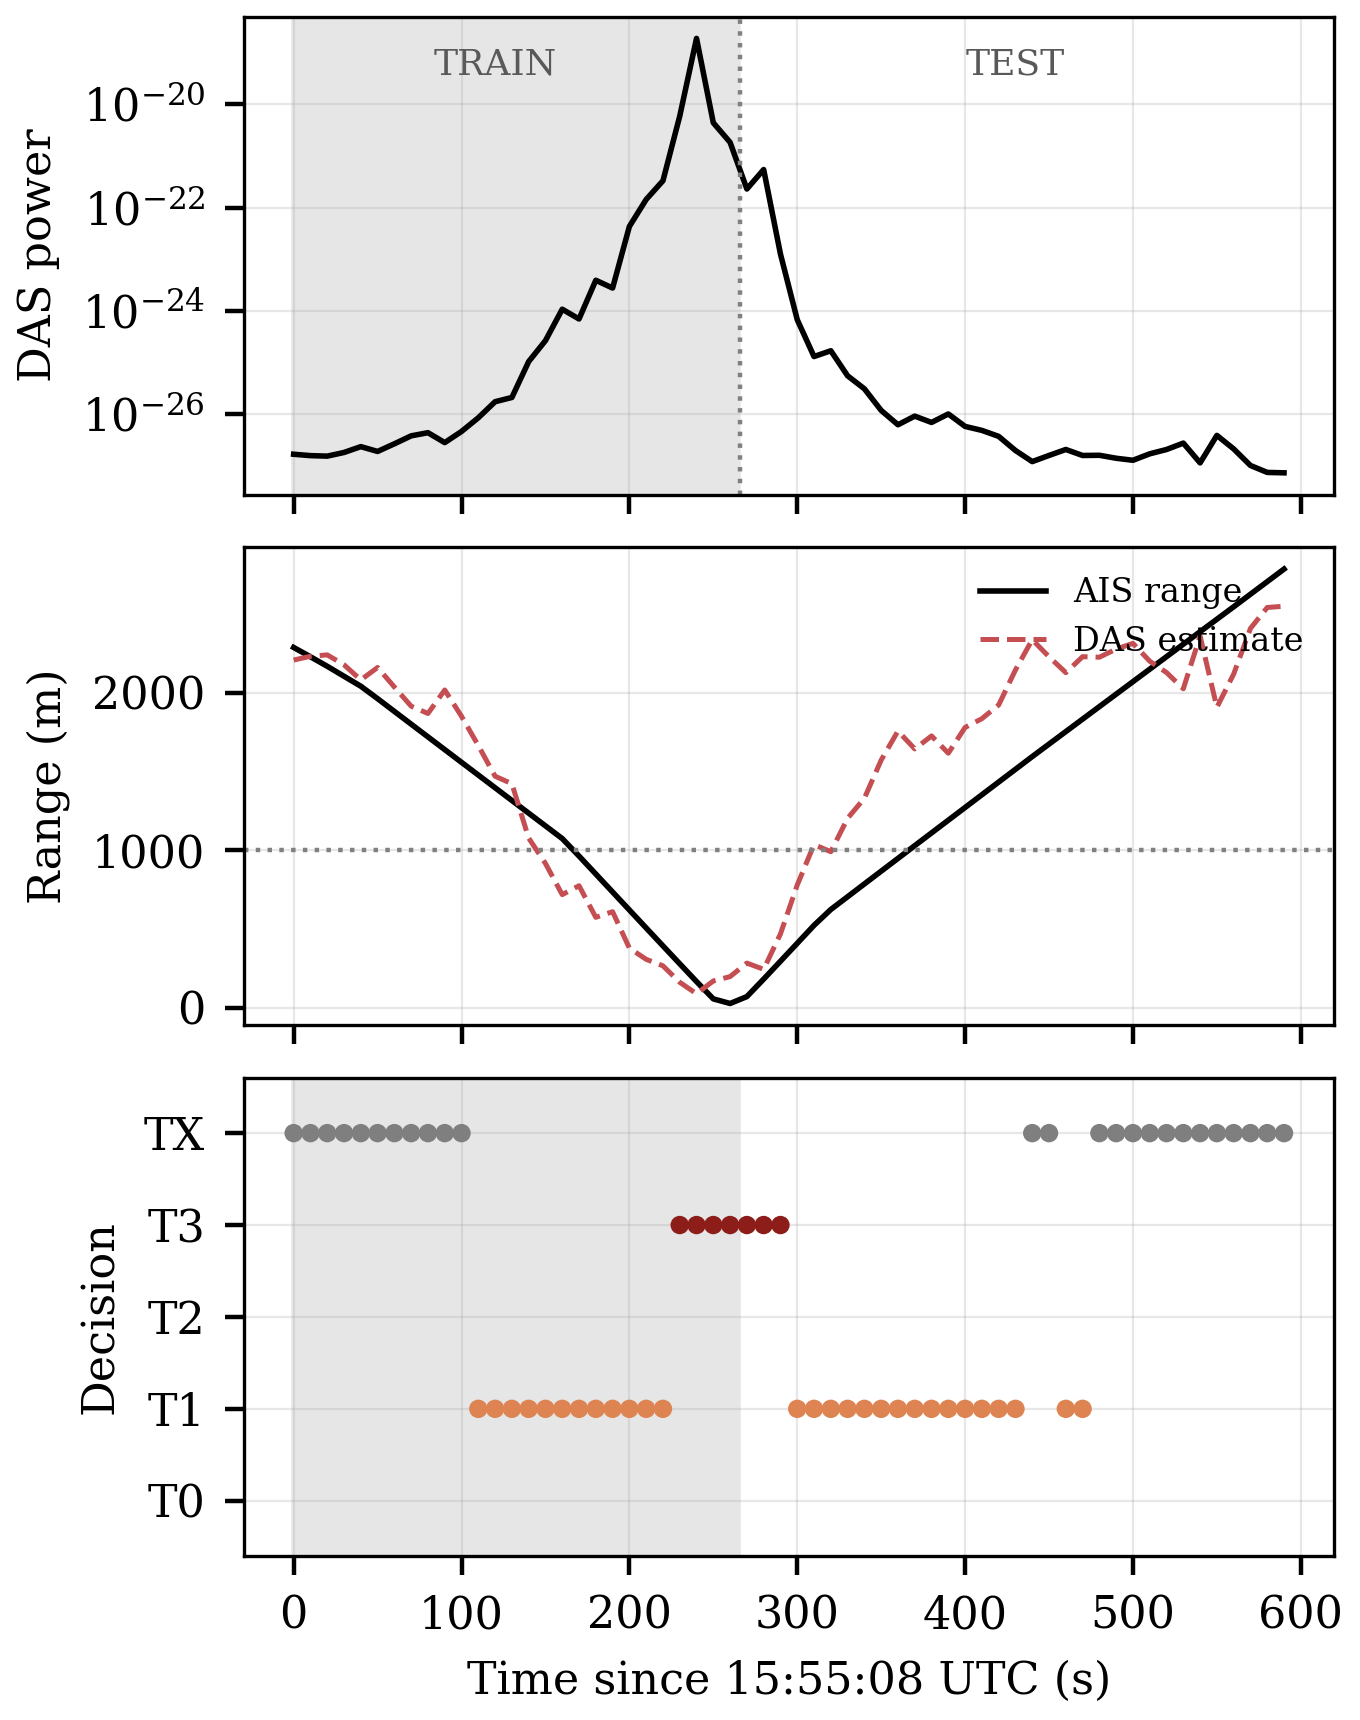
\includegraphics[width=0.45\textwidth]{figs/fig_transit.png}
\caption{Real transit response (Dataset A). Top: DAS window power spans seven
orders of magnitude. Middle: AIS ground-truth range and independent DAS range
inversion. Bottom: Graded decisions across the transit.}
\label{fig:transit}
\end{figure}

\subsection{Physical Detection on Real DAS}
\label{sec:detection-results}
Acoustic strain power exhibits a strong negative monotonic association with
vessel distance at Spearman $\rho = -0.948$ ($p = 1.4\times10^{-30}$,
$n=60$); equivalently, energy correlates at $\rho = +0.948$ with inverse
distance $1/d$. Evaluated against corridor boundaries on the
held-out leg, the coherent statistic achieves the detection AUC values
(area under the ROC curve) in Table~\ref{tab:auc}, reaching AUC $= 0.959$ (95\% CI $[0.887, 1.000]$) at 1~km.

\begin{table}[!t]
\caption{DAS-Only Detection Performance on Held-Out Leg ($n=33$)}
\label{tab:auc}
\centering
\footnotesize
\begin{tabular}{@{}cccc@{}}
\toprule
Corridor $R_c$ & Positives ($n$) & AUC & 95\% Bootstrap CI \\
\midrule
200~m & 2 & 0.871 & [0.790, 0.952] \\
500~m & 4 & 0.897 & [0.828, 0.966] \\
1000~m & 10 & \textbf{0.959} & [0.887, 1.000] \\
\bottomrule
\end{tabular}
\end{table}

Fig.~\ref{fig:horizon} reveals the physical detection horizon: coherent strain
$Z_{\mathrm{coh}}$ remains above threshold $\tau_P = 7$ out to 1.5~km.
Consequently, a physical-only detector triggers on transiting ships far outside
the security corridor, achieving recall 1.000 but precision 0.526
(Table~\ref{tab:methods}).

\begin{figure}[!t]
\centering
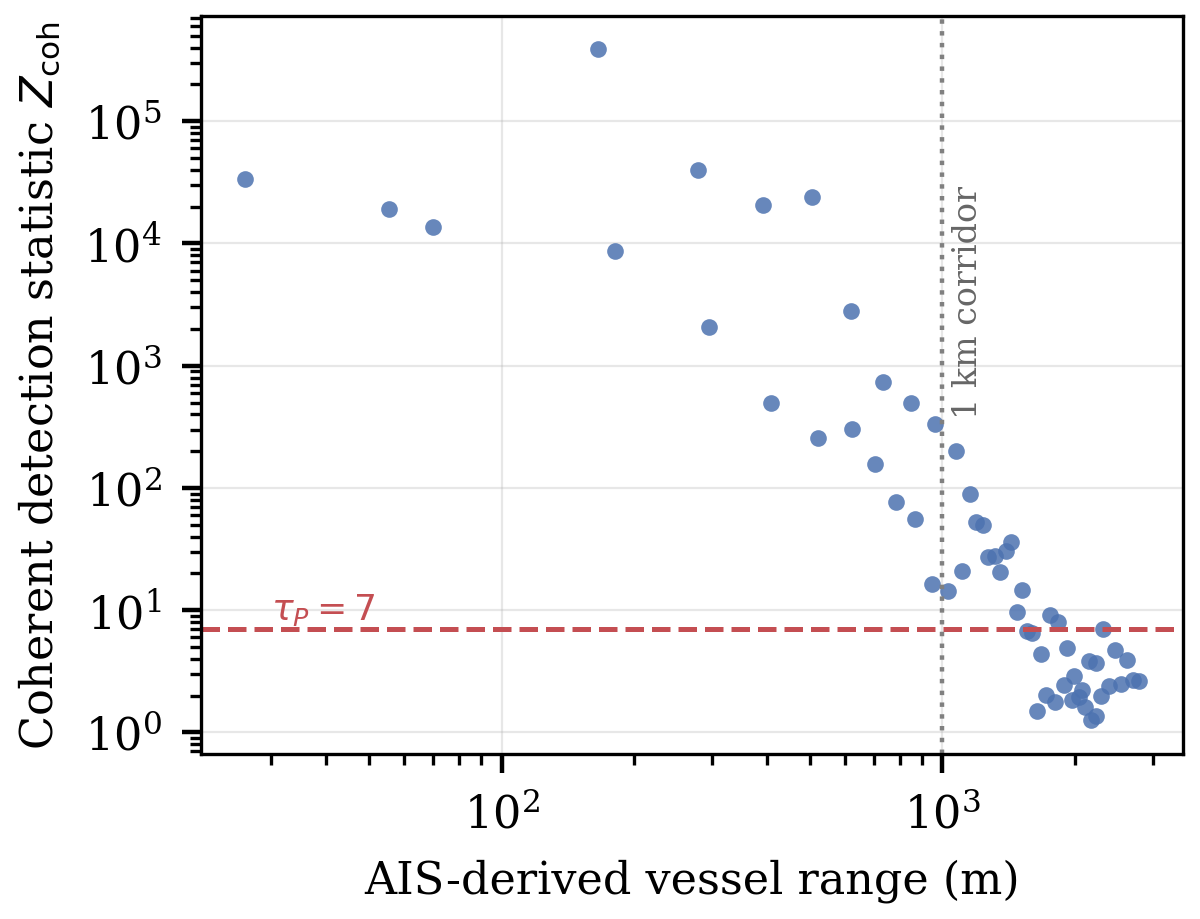
\includegraphics[width=0.42\textwidth]{figs/fig_horizon.png}
\caption{Coherent detection statistic against AIS range (Dataset A). The
physical detection boundary extends to roughly 1.5~km, well outside the 1~km
protection corridor.}
\label{fig:horizon}
\end{figure}

\subsection{Background Baseline and Threshold Calibration}
\label{sec:background}
On Dataset B, a static baseline drifts over 17 minutes, producing a 97.7\%
background detection exceedance rate. A rolling 200-second baseline stabilizes
the statistic at mean 4.15 (p95 6.01, max 6.99). Sweeping $\tau_P$ identifies
$\tau_P = 7$ as the minimal integer yielding zero background detection
exceedances (Fig.~\ref{fig:far}). Operating the full decision engine over
Dataset B (85 evaluated windows after 20-window rolling-baseline initialization)
produced \dstate{TX} in 85/85 windows and \textbf{zero} false escalations to
\dstate{T2}/\dstate{T3}, verifying fail-closed behavior when vessel
corroboration is absent. We term these \emph{background false alarms} (physical
detector exceedances on quiescent seafloor), distinct from \emph{environmental
escalations} (T2/T3 decisions during natural hydrodynamic forcing) and
\emph{vessel attribution errors} (incorrect vessel assignment).

\begin{figure}[!t]
\centering
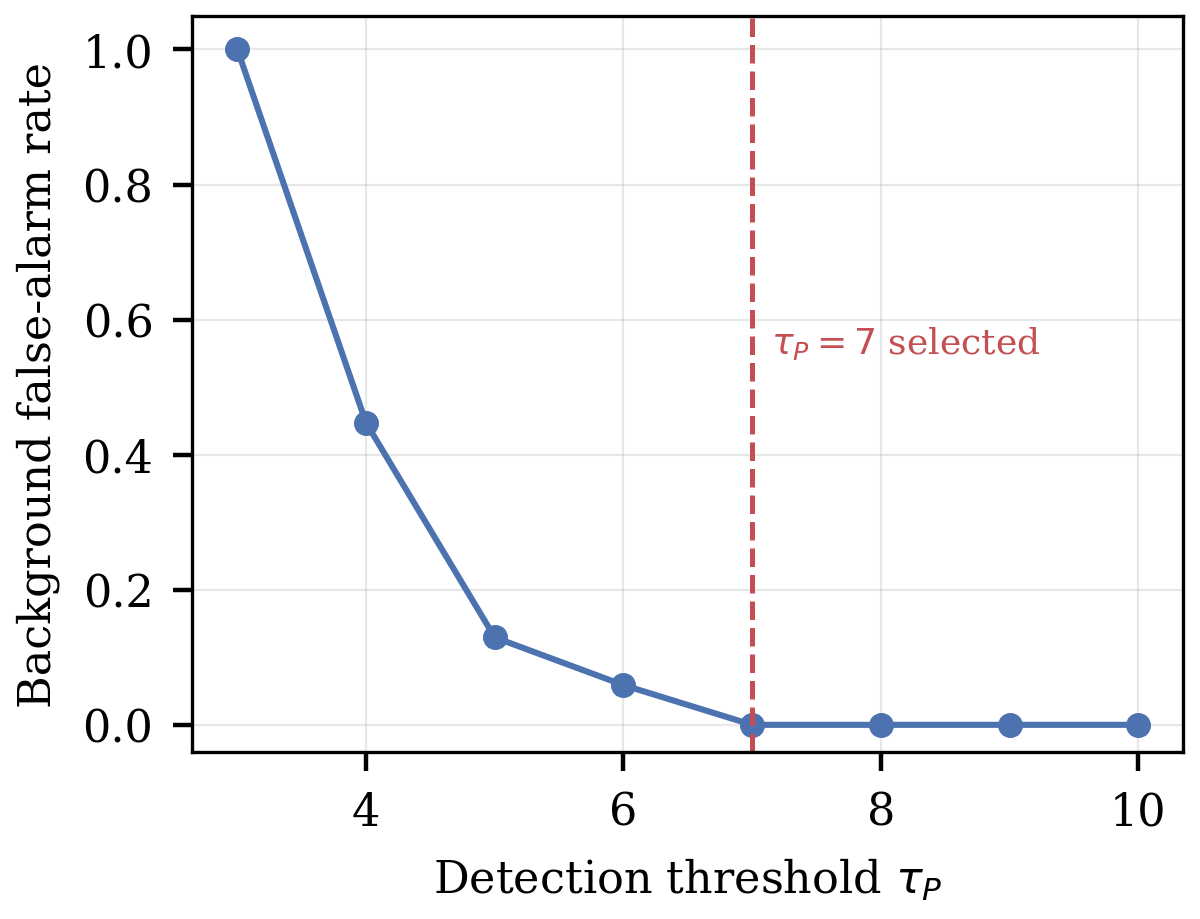
\includegraphics[width=0.42\textwidth]{figs/fig_far.png}
\caption{Background detection exceedance rate versus threshold on Dataset B
(85 evaluated windows, rolling baseline). The reference threshold $\tau_P=3$
produces 100\% exceedances; $\tau_P=7$ achieves zero.}
\label{fig:far}
\end{figure}

\subsection{Independent Real-DAS Environmental Validation}
\label{sec:oliktok-results}

Dataset C provides an independent multi-week stress test of the physical
detector under real Arctic oceanographic conditions. Over 215 continuous hourly
windows across 183 physical channels, the optical strain-rate field exhibited
stable seafloor coupling: mean integrated strain RMS was $550.85~\mathrm{nm/m/s}$
(median $553.59~\mathrm{nm/m/s}$), with spatial CV of 0.2349 and spatial Gini
coefficient of 0.1265. Over the 27.625-day deployment, temporal CV was 0.1239
with a negligible baseline drift slope of $+0.0188/\mathrm{hr}$ ($p = 0.8037$).
Skewness was $+0.1547$ and kurtosis was $-1.1625$.

\begin{table}[!t]
\caption{Dryad Oliktok Real Submarine DAS Environmental Validation}
\label{tab:oliktok}
\centering
\footnotesize
\setlength{\tabcolsep}{3pt}
\begin{tabular}{@{}>{\raggedright\arraybackslash}p{0.33\columnwidth}>{\raggedright\arraybackslash}p{0.26\columnwidth}>{\raggedright\arraybackslash}p{0.33\columnwidth}@{}}
\toprule
Metric & Verified Value & Scientific Interpretation \\
\midrule
Recording Duration & 27.625~d (215~hr) & Continuous deployment (Aug 24--Sep 20, 2023) \\
Spatial Channels & 183 physical ch & Ch 1088--3672 (8.8--30.0~km offshore) \\
Integrated Strain RMS & 550.85~nm/m/s & Mean noise floor (median 553.59) \\
Skewness / Kurtosis & $+0.1547$ / $-1.1625$ & Sub-Gaussian seafloor strain distribution \\
Temporal Stability (CV) & 0.1239 & Stable multi-week acoustic baseline \\
Baseline Drift Slope & +0.0188 / hr & Negligible systematic sensor drift ($p=0.8037$) \\
Spatial CV / Gini & 0.2349 / 0.1265 & Homogeneous seafloor coupling \\
$\rho$ vs Wave Height ($H_s$) & +0.3141 ($p=2.63\times10^{-6}$) & Statistically significant wave coupling \\
$r$ vs Wave Height ($H_s$) & +0.3370 ($p=4.31\times10^{-7}$) & Linear wave height correlation \\
$\rho$ vs Pressure Variance & +0.4951 ($p=1.07\times10^{-14}$) & Hydrodynamic seafloor pressure tracking \\
$r$ vs Pressure Variance & +0.4903 ($p=2.11\times10^{-14}$) & Linear bottom pressure correlation \\
Quiet Baseline (\dstate{T0}) & 93 / 215 (43.26\%) & Classified as quiescent seafloor baseline \\
Uncorroborated (\dstate{T1}) & 122 / 215 (56.74\%) & Escalated to environmental disturbance \\
Corroborated (\dstate{T2}/\dstate{T3}) & 0 / 215 (0.0\%) & No T2/T3 vessel escalations occurred \\
Degraded Stream (\dstate{TX}) & 0 / 215 (0.0\%) & Zero unforced fail-closed triggers \\
\bottomrule
\end{tabular}
\end{table}

\begin{figure}[!t]
\centering
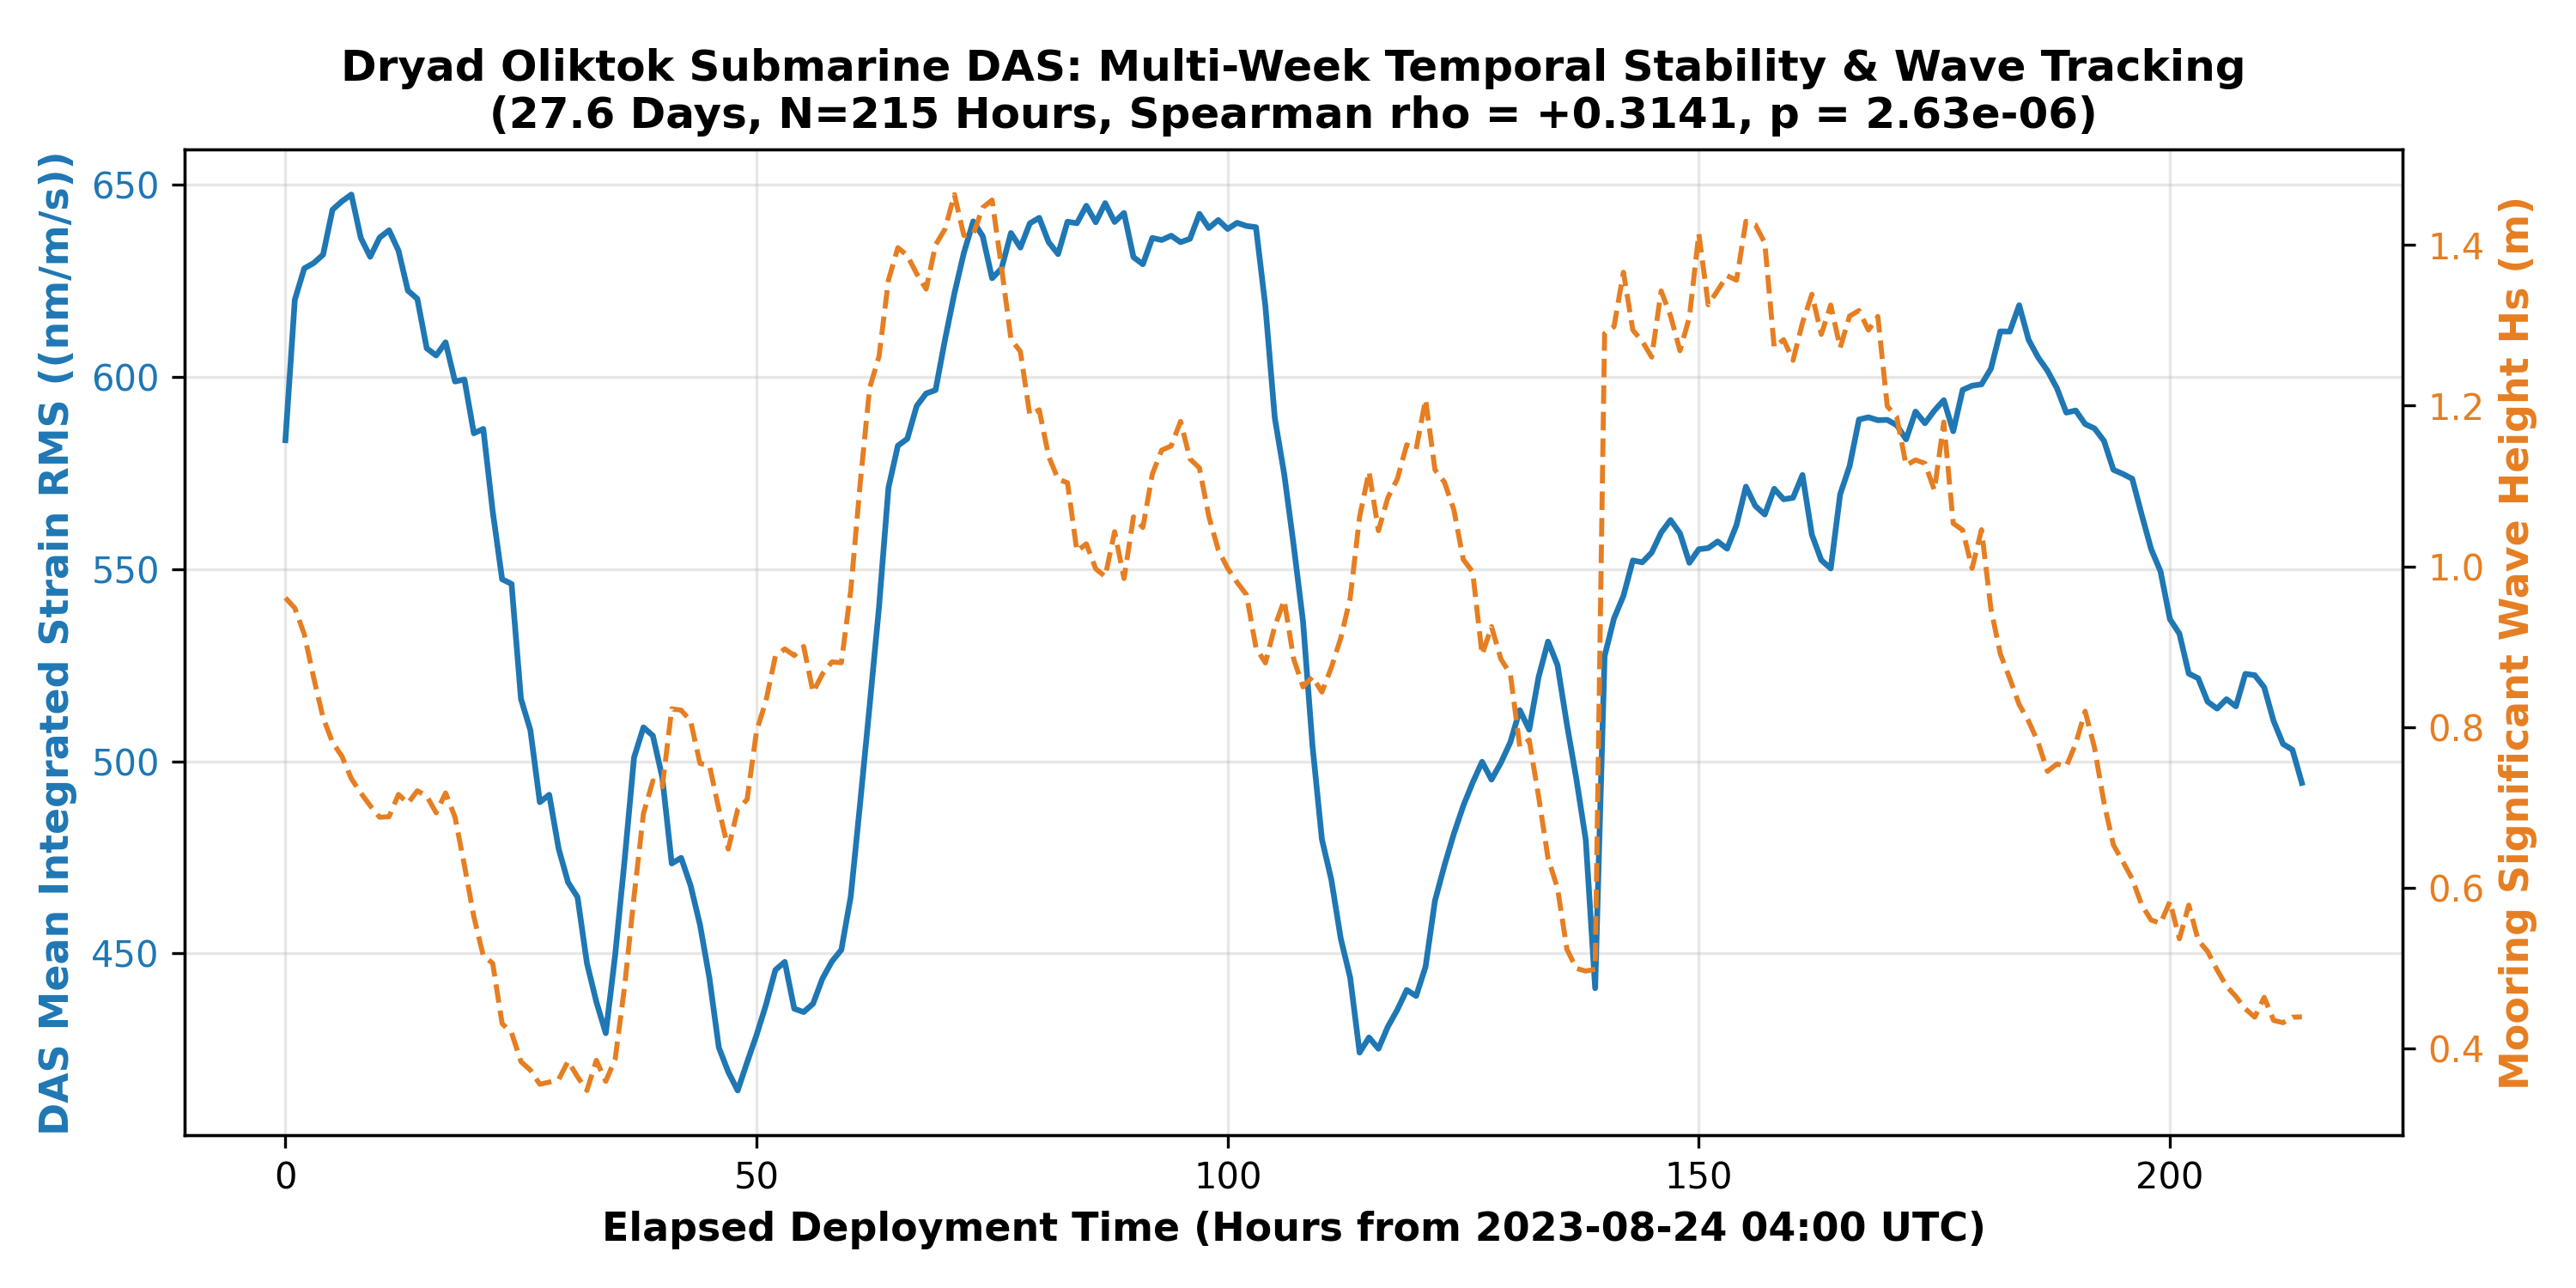
\includegraphics[width=0.45\textwidth]{figs/fig_oliktok_temporal.png}
\caption{Long-term temporal stability and environmental wave coupling on
Dataset C (Dryad Oliktok, 27.625 days). Seafloor acoustic energy tracks
independent ocean wave height without producing anomalous sensor drift.}
\label{fig:oliktok-temporal}
\end{figure}

The integrated strain exhibited statistically significant empirical associations
with independent oceanographic measurements: Spearman $\rho = +0.3141$
($p = 2.63\times10^{-6}$, Pearson $r = +0.3370, p = 4.31\times10^{-7}$) against
significant wave height $H_s$, and Spearman $\rho = +0.4951$
($p = 1.07\times10^{-14}$, Pearson $r = +0.4903, p = 2.11\times10^{-14}$) against
dynamic seafloor pressure variance. These correlations demonstrate empirical
monotonic association with surface hydrodynamics. They do not demonstrate
causal cable damage, as environmental records cannot establish causal physical
damage without annotated structural incident ground truth.

Processing Dataset C through the frozen decision pipeline produced 93
\dstate{T0} states (43.26\%) during calm periods, 122 \dstate{T1} states
(56.74\%) during wave excitation, and zero \dstate{T2}/\dstate{T3} states
(Table~\ref{tab:oliktok}). \textbf{No T2/T3 vessel-escalation decisions occurred
in the evaluated Oliktok environmental recording}, yielding an environmental
escalation rate of 0.0\%. Because Dataset C lacks vessel and AIS ground truth,
this finding is interpreted as an environmental robustness and false-escalation
avoidance observation rather than a vessel-attribution false-positive measurement.

\subsection{Decision Behavior on the Real Transit}
On Dataset A's held-out transit leg ($n=33$), the framework yielded 3 \dstate{T3},
16 \dstate{T1}, and 14 \dstate{TX} decisions (Table~\ref{tab:states}). The
gradations are physically consistent: \dstate{T3} occurs at close range
(mean 182.0~m, $C_P = 1.000, C_A = 0.738$); \dstate{T1} occurs at intermediate
ranges (mean 1084.0~m, $C_P = 0.977, C_A = 0.191$); and \dstate{TX} occurs at
far range (mean 2246.4~m) where acoustic energy subsides.

\begin{table}[!t]
\caption{Decision States on Held-Out Transit Leg ($n=33$)}
\label{tab:states}
\centering
\footnotesize
\begin{tabular}{@{}lccccc@{}}
\toprule
State & $n$ & Mean range (m) & $C_P$ & $C_A$ & $U$ \\
\midrule
\dstate{T3} & 3 & 182.0 & 1.000 & 0.738 & 0.094 \\
\dstate{T1} & 16 & 1084.0 & 0.977 & 0.191 & 0.361 \\
\dstate{TX} & 14 & 2246.4 & 0.096 & 0.066 & 0.225 \\
\bottomrule
\end{tabular}
\end{table}

\subsection{Method Comparison}
Table~\ref{tab:methods} evaluates the proposed framework against single-channel
and reduced baselines on the held-out transit ($R_c = 1000$~m). All methods
achieve precision 1.000 except physical-only (0.526).

\begin{table}[!t]
\caption{Method Comparison on Held-Out Transit Leg ($n=33$, $R_c=1000\,\mathrm{m}$)}
\label{tab:methods}
\centering
\footnotesize
\begin{tabular}{@{}lcccc@{}}
\toprule
Method & Accuracy & Precision & Recall & F1 \\
\midrule
behaviour\_only & 0.697 & 0.000 & 0.000 & 0.000 \\
physical + behaviour & 0.697 & 0.000 & 0.000 & 0.000 \\
physical-only & 0.727 & 0.526 & \textbf{1.000} & 0.690 \\
ais\_range\_only & 0.788 & 1.000 & 0.300 & 0.462 \\
association\_only & 0.788 & 1.000 & 0.300 & 0.462 \\
physical + spatial & 0.788 & 1.000 & 0.300 & 0.462 \\
physical + temporal & 0.849 & 1.000 & 0.500 & 0.667 \\
weighted (simple) & \textbf{0.909} & 1.000 & 0.700 & \textbf{0.824} \\
\textbf{Proposed (full)} & 0.788 & 1.000 & 0.300 & 0.462 \\
\bottomrule
\end{tabular}
\end{table}

The proposed method achieves F1 $= 0.462$, below simple weighted fusion (0.824)
and physical + temporal (0.667). In paired McNemar tests at $n=33$, differences
do not reach statistical significance ($p = 0.134$ vs weighted). The lower
escalation F1 reflects deliberate design conservatism: the full framework
requires high multi-channel corroboration before escalating, suppressing
marginal incursions.

\subsection{Ablation on Real Data}
Ablating individual components (Table~\ref{tab:ablation}) shows that removing
health weighting, uncertainty modeling, or adversarial checking changes no
decisions on the clean transit leg. This is expected: the health, uncertainty,
and adversarial modules are designed to activate under degraded or adversarial
conditions absent from this clean single-vessel transit; their contribution is
visible in the adversarial evaluation (Section~\ref{sec:adv-results}).
Removing behavioral scoring increases F1 from 0.462 to 0.571, whereas removing
spatio-temporal association collapses F1 to 0.000: association gating is doing
most of the work.

\begin{table}[!t]
\caption{Ablation Analysis on Held-Out Transit Leg ($n=33$)}
\label{tab:ablation}
\centering
\footnotesize
\begin{tabular}{@{}lccc@{}}
\toprule
Component Removed & Accuracy & Recall & F1 \\
\midrule
None (full proposed) & 0.788 & 0.300 & 0.462 \\
Sensor health weighting & 0.788 & 0.300 & 0.462 \\
Uncertainty model & 0.788 & 0.300 & 0.462 \\
Adversarial consistency check & 0.788 & 0.300 & 0.462 \\
Behavioral scoring & 0.818 & 0.400 & 0.571 \\
Spatio-temporal association & 0.697 & 0.000 & 0.000 \\
\bottomrule
\end{tabular}
\end{table}

\subsection{Adversarial Robustness and Evasion Rate}
\label{sec:adv-results}
The adversarial evaluation perturbed the vessel-side AIS channel across 10
genuine incursion windows while leaving the real fiber recording untouched.
Four attack families were evaluated at five severity levels (0.00, 0.25, 0.50,
0.75, 1.00): AIS range inflation, transponder suppression, timestamp offset,
and combined multi-vector evasion (Table~\ref{tab:adv}).

\begin{table}[!t]
\caption{Adversarial Evaluation on Real DAS (10 Incursion Windows)}
\label{tab:adv}
\centering
\footnotesize
\begin{tabular}{@{}lccccc@{}}
\toprule
\multirow{2}{*}{Attack Family} & \multicolumn{5}{c}{Consistency-Check Firing Rate by Severity} \\
\cmidrule(l){2-6}
 & 0.00 & 0.25 & 0.50 & 0.75 & 1.00 \\
\midrule
AIS range inflation & 0.00 & 0.10 & 0.30 & 0.40 & 0.60 \\
Transponder suppression & 0.00 & 0.20 & 0.50 & 0.90 & 1.00 \\
Timestamp manipulation & 0.00 & 0.00 & 0.00 & 0.00 & 0.00 \\
Combined multi-vector & 0.00 & 0.30 & 0.70 & 0.90 & 1.00 \\
\midrule
AER (all families) & 0.00 & 0.00 & 0.00 & 0.00 & 0.00 \\
\bottomrule
\end{tabular}
\end{table}

The adversarial evasion rate (AER), defined as the fraction of genuine-incursion
trials that collapse to \dstate{T0} under adversarial perturbation, was 0/200
(0.0) across all 20 attack cells ($4\ \text{families} \times
5\ \text{severities}$, 10 incursion windows each): within the implemented
vessel-side AIS/transponder threat model and tested severity range, 0/200
observed adversarial trials collapsed to \dstate{T0}. Mean uncertainty
rose from 0.225 to 0.436 under full attack, and the consistency check fired
monotonically with severity for range manipulation
(Fig.~\ref{fig:adversarial}). Crucially, the threat model covers vessel-side
telemetry manipulation only; this does not constitute complete cyber-physical
security against cable tampering or optical interrogator compromise.

\begin{figure}[t]
\centering
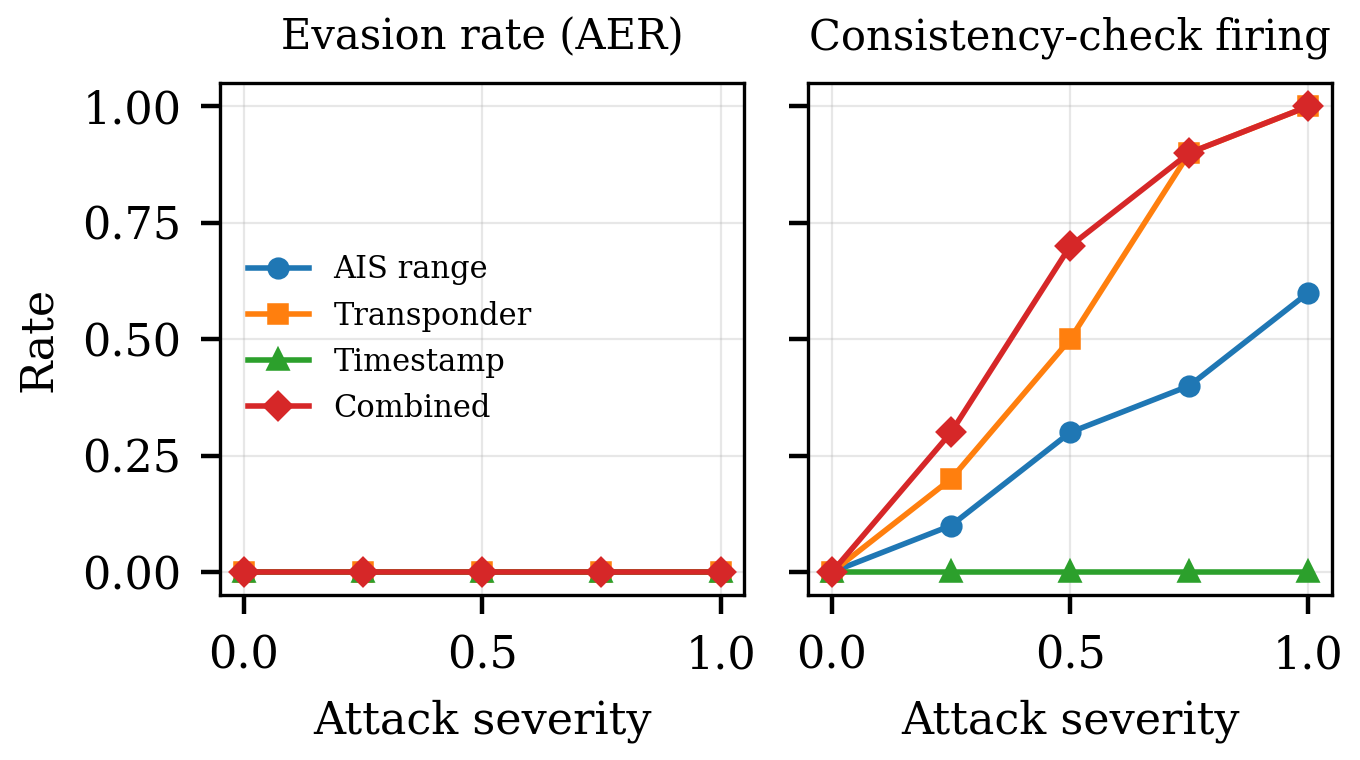
\includegraphics[width=\columnwidth]{figs/fig_adversarial.png}
\caption{Adversarial response on real DAS. Left: Adversarial evasion rate
remains 0.0 across all severities. Right: Range consistency check fires
monotonically for spatial attacks but remains inert under timestamp offsets.}
\label{fig:adversarial}
\end{figure}

\subsection{Robustness and Noise Sensitivity}
Under simulated optical channel dropout up to 90\%, escalation F1 remained
stable at 0.462 while \dstate{TX} declarations increased from 42.4\% to 78.8\%
and mean uncertainty rose from 0.279 to 0.485 (Fig.~\ref{fig:robustness}),
demonstrating graceful degradation. Conversely, extreme synthetic Gaussian noise artificially inflated $R$: high
unmodeled noise can displace windows from \dstate{TX}.

\begin{figure}[t]
\centering
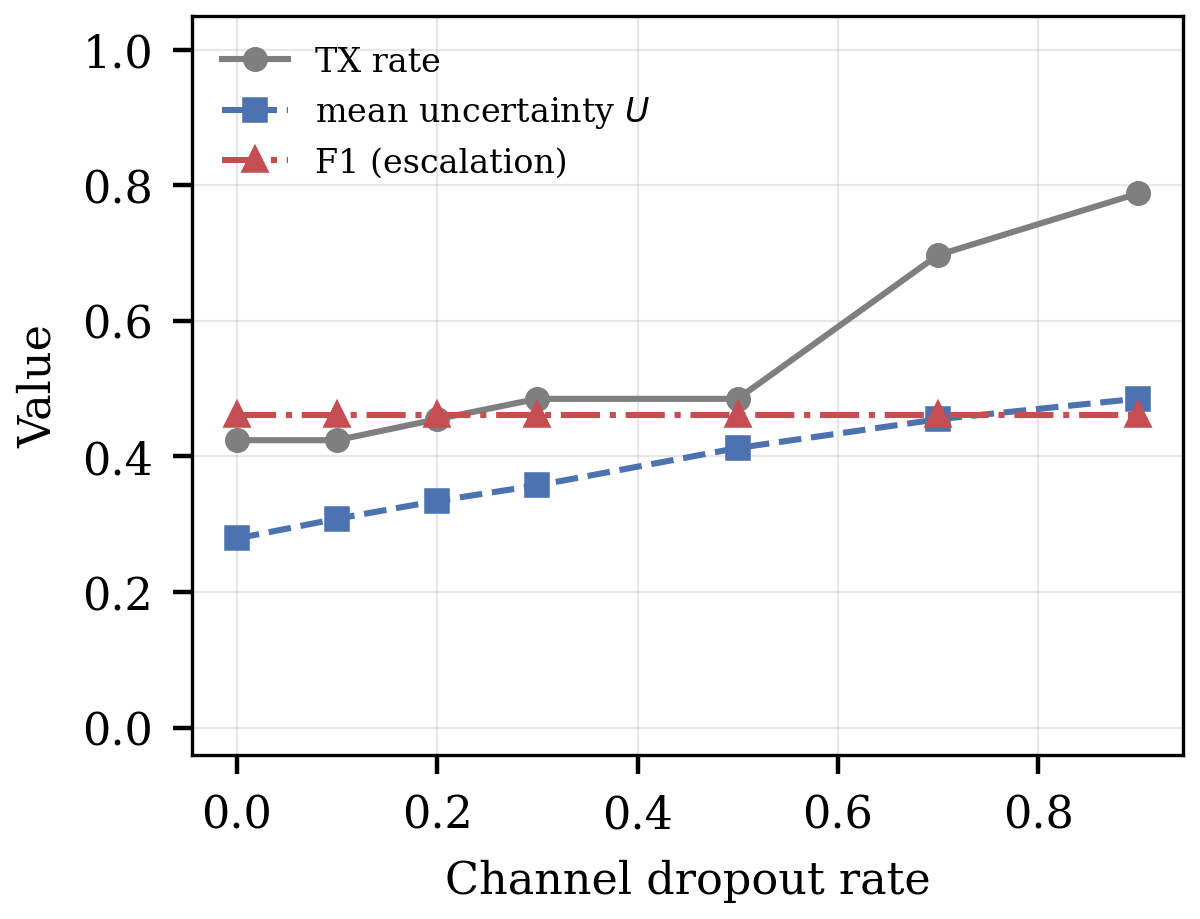
\includegraphics[width=0.95\columnwidth]{figs/fig_robustness.png}
\caption{Channel dropout robustness on real DAS. F1 remains constant while
\dstate{TX} declarations rise: the system degrades by asking for help, not by
guessing.}
\label{fig:robustness}
\end{figure}

\subsection{Calibration Assessment}
\label{sec:calibration}

\begin{figure}[t]
\centering
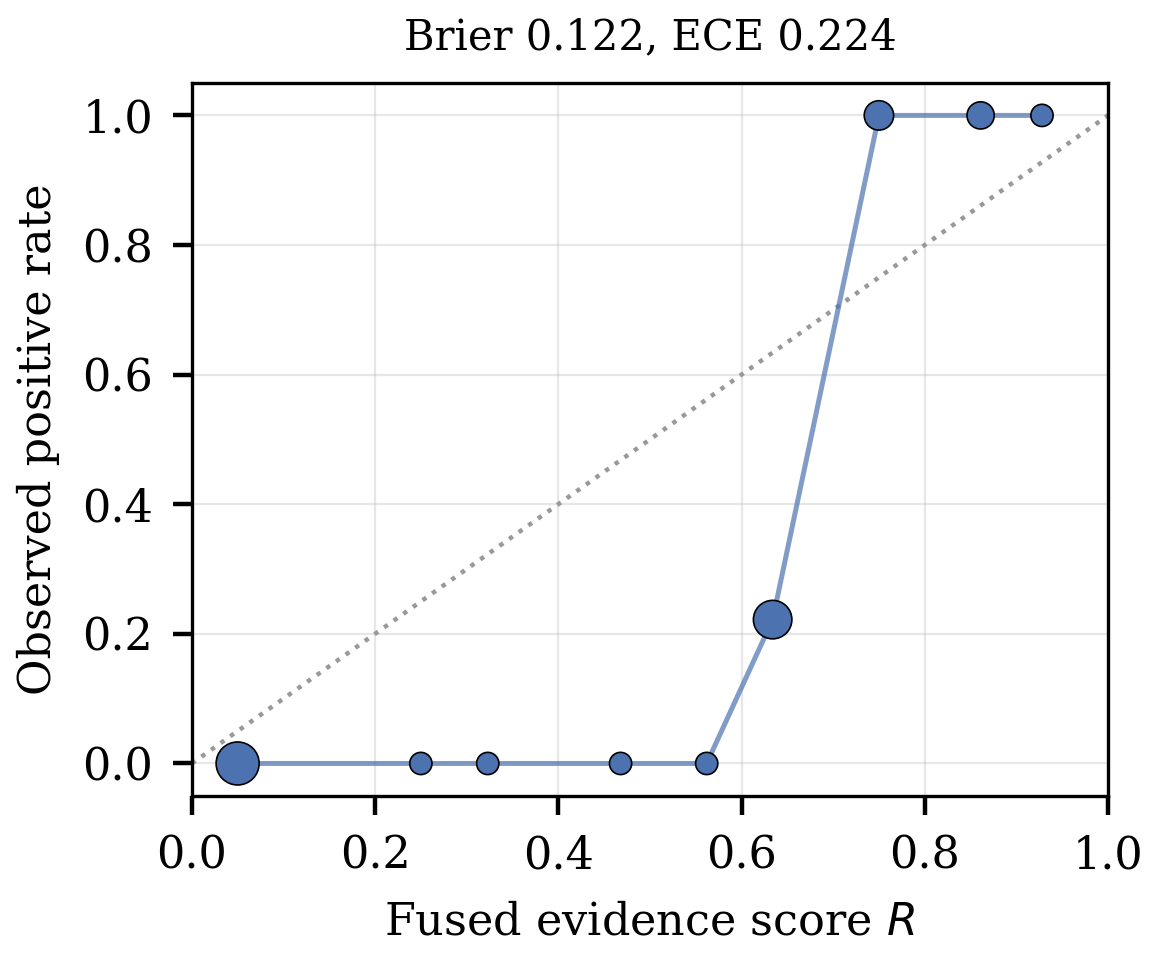
\includegraphics[width=0.95\columnwidth]{figs/fig_calibration.png}
\caption{Reliability calibration curve of fused score $R$ on the held-out
transit leg (Brier score $=0.122$; 10-bin expected calibration error (ECE)
$=0.224$). Marker area denotes bin sample occupancy.}
\label{fig:calibration}
\end{figure}

Evaluating fused evidence score $R$ as a predicted probability yields a Brier
score of 0.122 and a 10-bin Expected Calibration Error (ECE) of 0.224
(Fig.~\ref{fig:calibration}). While $R$ orders events effectively (high AUC),
it exhibits overconfidence in intermediate bins (0.2--0.6). Fused score $R$ is an operational reliability score, not a calibrated
posterior probability.

\subsection{Computational Performance}
\label{sec:performance}

\begin{table}[t]
\caption{Computational Latency (ms) and Throughput Profiling ($N=1{,}000$ Iterations)}
\label{tab:performance}
\centering
\setlength{\tabcolsep}{2pt}
\renewcommand{\arraystretch}{1.05}
\scriptsize
\begin{tabular}{@{}lrrrrr@{}}
\toprule
Stage & Mean & Median & P95 & Max & Throughput \\
\midrule
DAS Spectral Processing & 0.918 & 0.567 & 2.607 & 12.455 & 1{,}088.8~Hz \\
Spatio-Temporal Association & 0.031 & 0.020 & 0.051 & 2.147 & 32{,}083.4~Hz \\
Multimodal Evidence Fusion & 0.189 & 0.108 & 0.398 & 5.788 & 5{,}278.5~Hz \\
Decision State Machine & 0.009 & 0.005 & 0.010 & 2.564 & 111{,}271.8~Hz \\
\textbf{End-to-End Pipeline} & \textbf{8.289} & \textbf{6.230} & \textbf{19.526} & \textbf{63.437} & \textbf{120.6~Hz} \\
\bottomrule
\end{tabular}
\end{table}

Table~\ref{tab:performance} presents computational latency and throughput
benchmarked over $N=1{,}000$ iterations on an Intel processor. Mean end-to-end
pipeline latency was 8.289~ms (median 6.230~ms, p95 19.526~ms, throughput
120.6~Hz). Individual stages execute rapidly: DAS spectral processing averages
0.918~ms (1,088.8~Hz), spatio-temporal association averages 0.031~ms
(32,083.4~Hz), evidence fusion averages 0.189~ms (5,278.5~Hz), and the decision
state machine executes in 0.009~ms (111,271.8~Hz). All stages execute well within
the 10-second real-time window cadence.

\section{Controlled Simulation Results}
\label{sec:sim}

To assess edge cases unobserved in real datasets (sensor failure modes, multi-vessel
ambiguity, counter-evidence), we evaluated 2,200 seeded simulation trials across
22 controlled scenarios (S01--S22, 100 trials each). The proposed framework
produced 500 \dstate{T0}, 1{,}200 \dstate{T1}, 200 \dstate{T2}, 0 \dstate{T3},
and 300 \dstate{TX} states, achieving accuracy 0.4091 and escalation F1 0.2353
(Table~\ref{tab:sim-baselines}).

\begin{table}[!t]
\caption{Comparative Evaluation Across 2,200 Controlled Simulation Trials}
\label{tab:sim-baselines}
\centering
\footnotesize
\setlength{\tabcolsep}{3pt}
\begin{tabular}{@{}lccccc@{}}
\toprule
Method & Acc. & Prec. & Recall & F1 & TX Rate \\
\midrule
physical-only & 0.3182 & 0.0000 & 0.0000 & 0.0000 & 0.0000 \\
association\_only & 0.3182 & 0.0000 & 0.0000 & 0.0000 & 0.1364 \\
behaviour\_only & 0.3182 & 0.0000 & 0.0000 & 0.0000 & 0.1364 \\
physical + temporal & 0.5909 & 1.0000 & 0.4000 & \textbf{0.5714} & 0.1364 \\
weighted fusion & 0.4545 & 1.0000 & 0.2000 & 0.3333 & 0.0000 \\
\textbf{Proposed (full)} & 0.4091 & 1.0000 & 0.1333 & 0.2353 & 0.1364 \\
\bottomrule
\end{tabular}
\end{table}

Simulation ablation shows physical-only achieving F1 $= 0.000$, physical + spatial
F1 $= 0.4211$, physical + temporal F1 $= 0.5714$, and full fusion without health
F1 $= 0.3333$. As in the real evaluation, the proposed framework sacrifices
unconstrained recall to ensure fail-closed safety under sensor faults and
unsubstantiated alarms. Controlled simulation results evaluate synthetic models
and are not interchangeable with real-world validation.

\section{Discussion}

Synthesizing across real-data deployments and controlled simulations yields
three central conclusions.

First, the fail-closed safety property is validated on genuine submarine fiber.
Across 85 real deep-sea background windows (EMSO) and 215 continuous Arctic
environmental windows (Oliktok), the system produced zero false escalations to
\dstate{T2}/\dstate{T3}. Under four vessel-side adversarial attack families on
real DAS, zero incursion events collapsed to \dstate{T0}.

Second, physical detection is empirically decoupled from causal attribution.
Because acoustic waves propagate through water and seabed sediments, large
vessels excite fiber channels out to 1.5~km. Physical-only monitoring triggers
continuous false alarms during normal transit. Robust protection requires
spatio-temporal association and independent range verification.

Third, the lower escalation F1 scores (0.462 on real data, 0.235 on simulation,
evaluated independently) come from an explicit engineering choice. The
framework prioritizes uncertainty awareness, health gating, and fail-closed
security over optimistic classification.

\section{Limitations}
\label{sec:limitations}

\begin{enumerate}
\item \textbf{Absence of vessel ground truth in Oliktok:} Dataset C contains no
vessel transponder logs or AIS data; its results validate environmental
robustness and escalation avoidance, not vessel classification accuracy.
\item \textbf{Absence of causal cable damage ground truth:} No dataset
contains verified structural cable damage incidents; attribution claims cannot
be causally verified against physical breaks.
\item \textbf{1D proximity constraint in Marlinks:} Dataset A provides 1D
distance $y$ rather than complete 2D geographic coordinates or polyline geometry.
\item \textbf{Unresolved non-vessel mechanical disturbances ($H_3$):}
Distinguishing vessel anchoring from benthic dredging or geological motion
remains unvalidated on real submarine fiber.
\item \textbf{Non-interchangeability of simulation and real data:} Synthetic
simulation provides controlled edge cases but cannot substitute for in-situ
oceanographic propagation.
\item \textbf{Vessel-side adversarial scope:} The threat model is restricted to
AIS telemetry falsification and does not cover physical fiber tampering, optical
interrogator compromise, or network eavesdropping.
\item \textbf{Hardware prototype boundary:} Benchtop hardware validation is not
equivalent to submerged maritime deployment.
\item \textbf{Frequency-domain DAS limitations:} Processed spectral band powers
do not equal full-bandwidth high-frequency optical phase waveforms.
\item \textbf{Correlation versus causation:} Oceanographic wave correlations
demonstrate natural hydrodynamic coupling, not causal cable degradation.
\item \textbf{Geographic diversity limitations:} Validated data represent
three localized regions (North Sea, Ionian Sea, Beaufort Sea), which do not
encompass global variations in seabed geology, water depth, and maritime traffic.
\end{enumerate}

\section{Reproducibility}

All reported results derive deterministically from executable scripts and frozen
manifests. Source data files are verified via SHA-256 hashes: Dataset A
(\texttt{46f5d2838342}), Dataset B (\texttt{8af2afac41b9}), Dataset C
(\texttt{5fa69e4cf90a}), and companion along-cable file (\texttt{6f9927adbfea}).
Random number generators use master seed 42. Execution is replicated via
\texttt{scripts/run\_real\_evaluation.py} and
\texttt{scripts/run\_phase3\_validation.py}. No reported value was manually altered.

\section{Conclusion and Future Work}
\label{sec:conclusion}

This paper presented an uncertainty-aware multimodal evidence fusion framework
for evaluating vessel-associated subsea cable disturbances. Evaluated across
three real submarine DAS deployments spanning the North Sea, Mediterranean, and
Arctic Ocean, the framework demonstrates that physical disturbance detection
can be decoupled from vessel association and causal attribution. Across 27.6
days of Arctic environmental DAS data and 1,050~s of deep-sea baseline data,
the system achieved zero false escalations to \dstate{T2}/\dstate{T3}, while
maintaining an adversarial evasion rate of 0.0 against vessel-side AIS
manipulation. The adversarial security claims are formally bounded in scope, escalation F1
is reported honestly against unconstrained fusion (evaluated independently on
real and simulated data), and every claim is checked against executable
artifacts.


\subsection{Future Work: Hardware Validation Scope}
\label{sec:hardware}

The physical ESP32--MPU6050 testbed described in early project plans was not
constructed; no hardware metrics appear in this paper. We formalize its
experimental scope for future reproducibility.

\textbf{Configuration:} Five ESP32 microcontrollers paired with MPU6050
six-axis inertial measurement units (IMUs) sampled at 10~Hz, deployed along a scaled
conduit in a hydrodynamic test tank, communicating over Wi-Fi/LoRa to an edge
aggregator running the decision engine.

\textbf{Intended Measurements:} (i) Real-world communication packet loss and
radio latency; (ii) physical sensor disconnects and saturation faults; and
(iii) empirical verification of edge decision execution under electrical noise.

\textbf{Claim Boundaries:} A benchtop IMU testbed cannot validate ocean
acoustic propagation or deep-sea vessel dynamics; it serves strictly to test
embedded firmware execution under controllable physical hardware faults.

\begin{thebibliography}{00}
\bibitem{b1} N. Srikanth and S. S. Rao, ``Subsea cable health monitoring system,'' in \textit{Proc. IEEE Asian Conf. Energy, Power Transp. Electrific. (ACEPT)}, 2017, doi: 10.1109/ACEPT.2017.8168582.
\bibitem{b2} A. Tudorache, J. Timmerberg, S. Mylvaganam, M. Stender, F. Xiaozhong, and L. Zhu, ``Subsea cable tracking using data fusion of signals from array of sensing coils,'' in \textit{Proc. 30th Annu. Conf. Eur. Assoc. Educ. Electr. Inf. Eng. (EAEEIE)}, 2021, doi: 10.1109/EAEEIE50507.2021.9530924.
\bibitem{b3} A. P. Balasuriya and T. Ura, ``Autonomous underwater vehicles for submarine cable inspection: Experimental results,'' in \textit{Proc. IEEE Int. Conf. Syst., Man, Cybern. (SMC)}, 2001, doi: 10.1109/ICSMC.2001.969841.
\bibitem{b4} W. Tang, D. Flynn, and V. Robu, ``Sensing technologies and artificial intelligence for subsea power cable asset management,'' in \textit{Proc. IEEE Int. Conf. Prognostics Health Manage. (ICPHM)}, 2021, doi: 10.1109/ICPHM51084.2021.9486586.
\bibitem{b11} E. E. Ramirez-Torres \textit{et al.}, ``Vessel Detection and Localization Using Distributed Acoustic Sensing in Submarine Optical Fiber Cables,'' \textit{IEEE J. Sel. Topics Appl. Earth Observ. Remote Sens.}, 2026, doi: 10.1109/JSTARS.2026.3716768.
\bibitem{b12} E. E. Ramirez-Torres \textit{et al.}, ``Marlinks-NS DAS: Dataset for Vessel Detection and Distance Estimation Using Distributed Acoustic Sensing in Submarine Optical Fiber Cables,'' Zenodo, 2026, doi: 10.5281/zenodo.15611778.
\bibitem{b13} E. E. Ramirez-Torres \textit{et al.}, ``A Distributed Acoustic Sensing Dataset for Vessel Detection and Localization in Submarine Cable Protection,'' arXiv:2607.28306, 2026, doi: 10.48550/arXiv.2607.28306.
\bibitem{b14} L. Thiem, M. Vaupel, S. Wienecke, J. Eidsvik, K. Taweesintananon, and M. Landr{\o}, ``Tracking ships with submarine cables: Unsupervised arrival time detection and event localization using distributed acoustic sensing,'' Zenodo, 2026, doi: 10.5281/zenodo.18851481.
\bibitem{b15} J. Davis \textit{et al.}, ``Distributed acoustic sensing observations of ocean surface waves and seafloor pressure in the Arctic,'' Dryad Digital Repository, 2024, doi: 10.5061/dryad.brv15dvnz.
\bibitem{b5} P. Prasad, V. Vatsal, and R. Roy Chowdhury, ``Maritime Vessel Route Extraction and Automatic Information System (AIS) Spoofing Detection,'' in \textit{2021 Int. Conf. Advances in Electrical, Computing, Communication and Sustainable Technologies (ICAECT)}, 2021, doi: 10.1109/ICAECT49130.2021.9392536.
\bibitem{b6} E. d'Afflisio, P. Braca, and P. Willett, ``Malicious AIS spoofing and abnormal stealth deviations: A comprehensive statistical framework for maritime anomaly detection,'' \textit{IEEE Trans. Aerosp. Electron. Syst.}, vol. 57, no. 5, pp. 3151--3165, 2021, doi: 10.1109/TAES.2021.3090715.
\bibitem{b7} J. Coleman, F. Kandah, and B. Huber, ``Behavioral Model Anomaly Detection in Automatic Identification Systems (AIS),'' in \textit{2020 10th Annual Computing and Communication Workshop and Conference (CCWC)}, 2020, pp. 481--487.
\bibitem{b8} Z. Deng and J. Wang, ``A Novel Evidence Conflict Measurement for Multi-Sensor Data Fusion Based on the Evidence Distance and Evidence Angle,'' \textit{Sensors}, vol. 20, no. 2, p. 381, 2020, doi: 10.3390/s20020381.
\bibitem{b9} F. Xiao and B. Qin, ``A Weighted Combination Method for Conflicting Evidence in Multi-Sensor Data Fusion,'' \textit{Sensors}, vol. 18, no. 5, p. 1487, 2018, doi: 10.3390/s18051487.
\bibitem{b10} Q. Liang, Z. Liu, and Z. Chen, ``A Networked Method for Multi-Evidence-Based Information Fusion,'' \textit{Entropy}, vol. 25, no. 1, p. 69, 2023.
\end{thebibliography}

\end{document}
